\documentclass[a4paper]{article}

\usepackage[utf8]{inputenc}
\PassOptionsToPackage{hyphens}{url} % zodat url's ook afgekapt worden
\usepackage{hyperref}
\usepackage[dutch]{babel}
\usepackage{graphicx}
\usepackage{algorithm}
\usepackage{algorithmic}
\usepackage{mathtools}
\usepackage{tikz}
\usepackage{tocbibind}
\usepackage{float}
\usepackage{framed}
\usepackage{parskip}
\usepackage{listings}
\usepackage{color}
\usepackage{pdfpages}
\usepackage{pdflscape}
\usepackage{todonotes}

\title{Software Engineering Analyse: \\ Glasbedrijf Software}
\author{Vincent Drozdzyniak 1334231 \\ Hendrik Lievens 1130921 \\ Martijn Maes 1131102 \\ Reinaert Van de Cruys 1334947 \\ Michiel Vanmunster 1334724 \\ Jens Vannitsen 1334039}
\date{\today}

\begin{document}
\maketitle

\section{Probleemstelling}
Roelants Glas is een lokale glasspecialist die nood heeft aan een algemeen beheersysteem. Alle administratie gebeurt op dit moment aan de hand van een combinatie van Excel bestanden en doordrukpapier. De volledige workflow vanaf informeren tot plaatsing moet gedigitaliseerd worden om zo de kans op fouten te verminderen en algemene efficiëntie te verhogen.

Deze workflow start met het informeren van de klanten van Roelants Glas. Daarna wordt een prijs gecalculeerd en een offerte gestuurd naar de klant. Indien de klant akkoord gaat, wordt het glas afgehaald, geleverd of geplaatst. Indien het om een plaatsing gaat, moet een personeelslid ter plaatse de opgegeven afmetingen gaan controleren. Indien er een mismatch is tussen de gegevens van de klant en die van de opmeter, herstart de workflow vanaf de calculatie fase.

Wanneer de gegevens overeen komen, wordt er beslist of het glas uit stock komt, geproduceerd moet worden of besteld moet worden bij een leverancier. Hierna wordt een plaatsingsbon door de software gegenereerd waar alle belangrijke informatie over de bestelling op staat, waaronder de gevraagde producten, het aantal vakwerkers vereist voor de levering en eventuele extra benodigdheden zoals een kraan.

Nadat de bestelling afgehaald, geleverd of geplaatst is, produceert de software een voorstel tot facturatie. Hier moet het mogelijk zijn om de prijs nog aan te passen indien er fouten zijn gebeurd bij eventuele (ver)plaatsing. De workflow eindigt met de opvolging van de betaling.

\section{Requirements analyse}
\begin{enumerate}
	\item Het systeem moet toelaten om aanvragen van offertes te registreren, aan te passen en te verwijderen.
	\item Het systeem moet standaardprijzen voor offertes kunnen genereren.
	\item Het systeem moet toelaten om korting te geven op offertes (of de prijs te verhogen).
	\item Het systeem moet de marge tussen de aankoopprijs en een gegeven bedrag kunnen visualiseren.
	\item Het systeem moet toelaten om een offerte te genereren op basis van een aanvraag en een prijs.
	\item Het systeem moet toelaten om offertes te verzenden.
	\item Het systeem moet toelaten om de status van een project in te kunnen stellen, aan te kunnen passen en op te kunnen vragen.
	\item Het systeem moet toelaten om stock bij te houden.
	\item Het systeem moet toelaten om een productiebon te maken.
	\item Het systeem moet toelaten om een bestelling te maken.
	\item Het systeem moet toelaten een factuur te genereren.
	\item Het systeem moet toelaten de facturatie op te volgen.
	\item Het systeem moet toelaten voor opmeters schema's te tonen op locatie.
	\item Het systeem moet toelaten voor opmeters om de maten in te geven op locatie.
	\item Het systeem moet toelaten klantendossiers aan te maken, te bewerken en te verwijderen.
    \item Het systeem moet toelaten inkooporders aan te maken aan de hand van de verkooporders.
    \item Het systeem moet uitgebreide terugzoekmogelijkheden toelaten.
    \item Het systeem moet statistieken voor omzet kunnen genereren.
    \item Het systeem moet toelaten om te berekenen hoe een reeks figuren uit zo weinig mogelijk glasplaten gesneden kan worden. 
\end{enumerate}

\clearpage
\section{URPS}
\subsection{Usability}
De UI is een zeer belangrijk onderdeel van de software. Aangezien het om een beheersysteem gaat, staat of valt de kwaliteit van het pakket met de overzichtelijkheid waarmee informatie wordt weergegeven en de vlotheid waarmee de software gebruikt kan worden. Daarom is ook consistentie van groot belang. 

De workflow die bij Roelants Glas gebruikt wordt, zal volledig door de software ondersteund worden. Dit houdt in de dat de bestaande fases in de workflow in dezelfde volgorde in de software zullen worden overgenomen. Dit heeft het dubbele voordeel dat we een workflow hanteren die reeds langdurig beproefd is en meteen ook de werking van de software herkenbaar maken voor de personeelsleden van Roelants Glas, wat de overstap vergemakkelijkt.

In de software zal uitgebreid gebruik gemaakt worden van standaardwaarden die indien gewenst kunnen worden aangepast. Deze techniek verhoogt de flexibiliteit zonder de workflow te vertragen of te bemoeilijken. Gebruikers zullen ook niet zelf moeten controleren of bepaalde stappen in de workflow zijn misgegaan, de software zal steeds automatisch waarschuwen bij onverwachte situaties.

\subsection{Reliability}
De klant- en projectgegevens worden op een database opgeslagen die fysiek gescheiden is van de client computers. Hierdoor blijven de gegevens veilig indien een van de clients faalt. Met bepaalde tussenperiodes gebeurt er ook een auto-save op de clients, frequent lokaal en minder frequent naar de database.

\subsection{Performance}
Op het vlak van performantie zijn er geen echte vereiste, zolang alle acties een snelle respons krijgen ($<$ 2 sec.). Op die manier komt de gebruiksvriendelijkheid nooit onder de performance te lijden. Door gebruik te maken van een externe database, kunnen er eenvoudig meerdere clients ondersteund worden en is de software ook beter schaalbaar.

\subsection{Supportability}
Door gebruik te maken van configuratiebestanden, kunnen instellingen makkelijk aangepast worden zonder een nieuwe versie uit te moeten brengen. Ook zal het systeem modulair en volgens goede design principes worden ontwikkeld om het eenvoudig uitbreidbaar te houden.

\subsection{Packaging}
Het plan is om de software als download beschikbaar te stellen op een bijhorende productwebsite. Dit lijkt ons de beste optie, aangezien serverkosten steeds lager worden, we redelijkerwijs een internetverbinding met voldoende bandbreedte bij de klant kunnen veronderstellen en we via deze weg ook eenvoudig updates kunnen uitbrengen, wat de supportability verhoogt.

\subsection{Legal}
De software zal allerlei gevoelige data beheren, waaronder gegevens van het bedrijf zelf, zoals een personeelsbestand en een register van inkomsten en uitgaven, maar ook gegevens van externe partijen, zoals rekeningnummers van klanten en leveranciers. Enkel bevoegde mensen binnen het bedrijf mogen toegang krijgen tot deze gegevens.

\section{Kost}
We schatten zo'n 30 dagen per persoon nodig te hebben, dit komt neer op zo'n 180 werkdagen.

\section{Mockups}
\begin{figure}[H]
  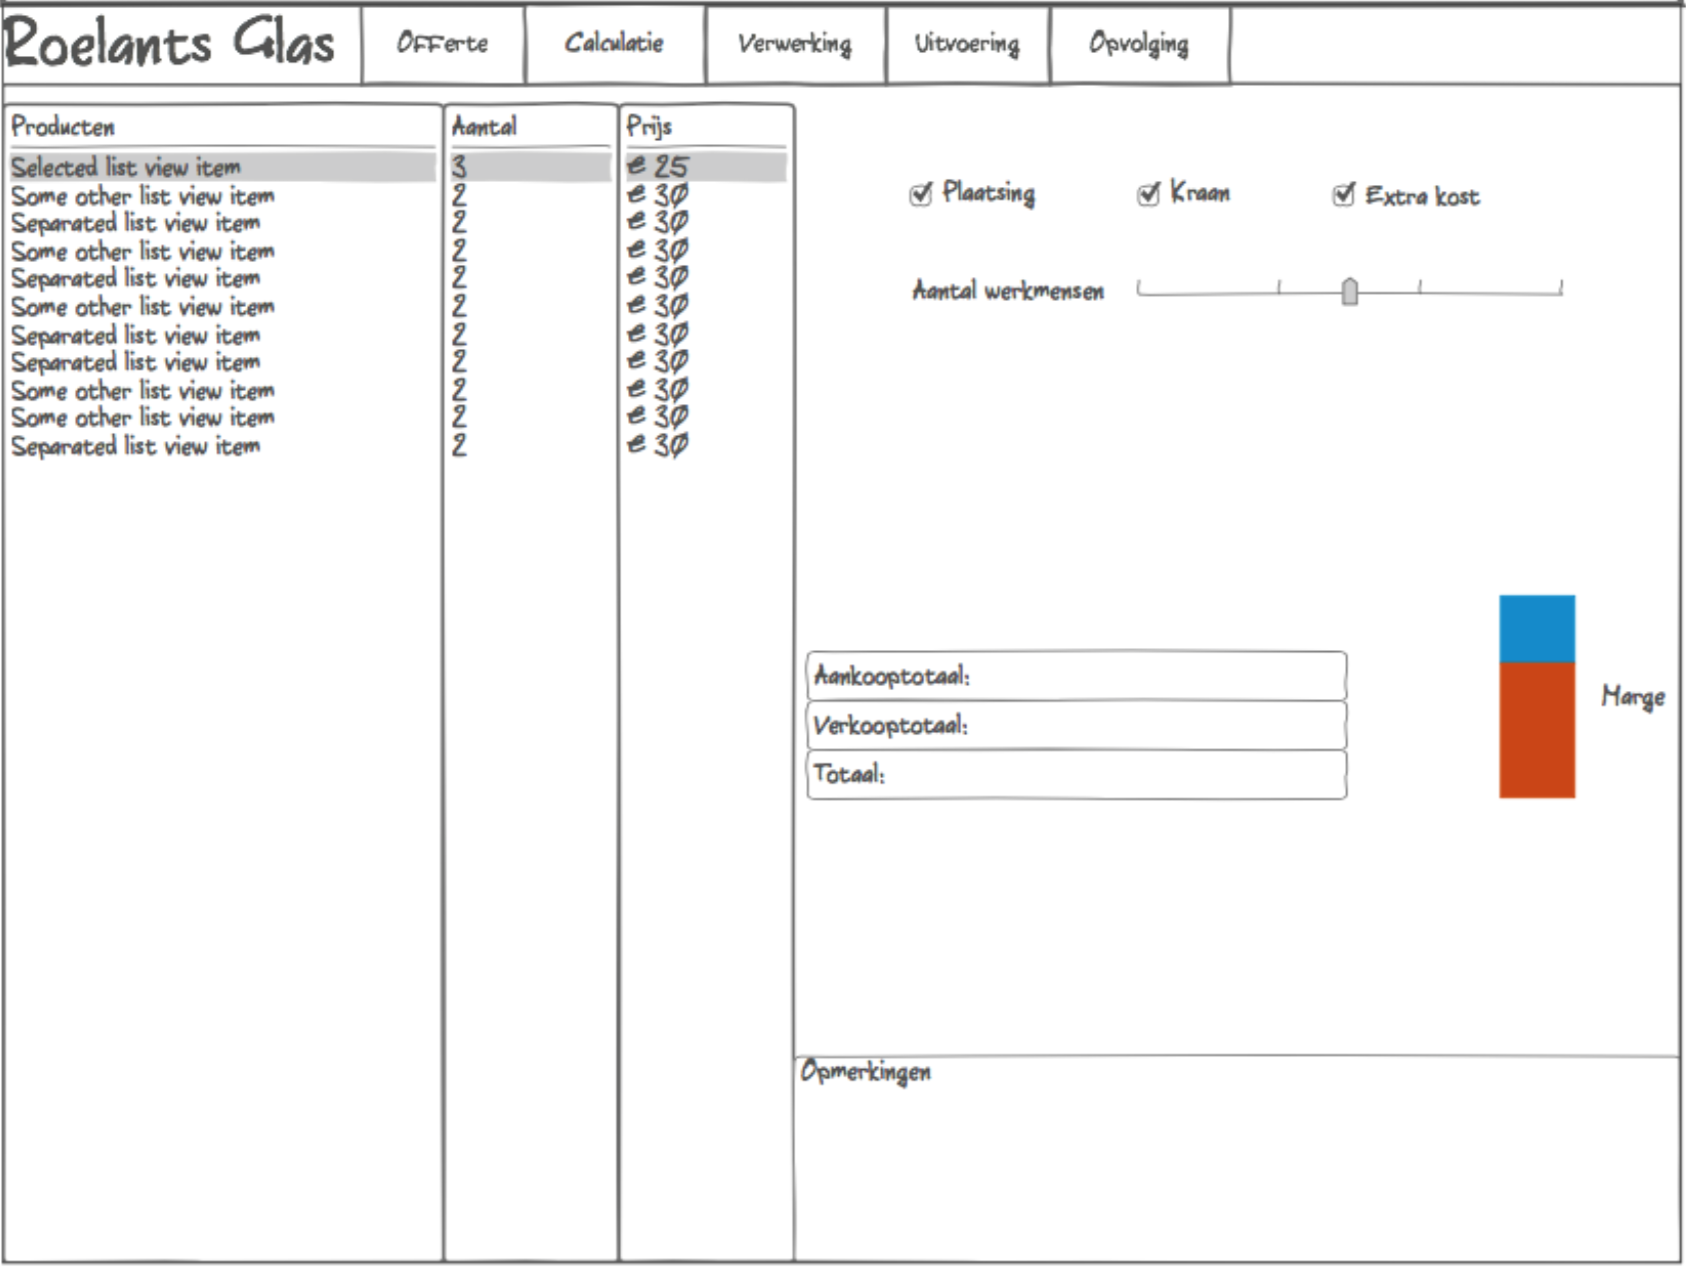
\includegraphics[width=\textwidth]{Mockup.png}
%  \caption{}
%  \label{fig:}
\end{figure}


\end{document}